\documentclass[12pt,titlepage,a4paper]{article}
%\documentclass[a4paper,fontsize=13pt]{scrartcl}

\usepackage{vntex}
%\usepackage{helvet} %set font Helvetica

%\usepackage{times} %set font Times New Roman
%\renewcommand{\familydefault}{\sfdefault} %set font Sans Serif

%\usepackage[english,vietnam]{babel}
%\usepackage[utf8]{inputenc}

\usepackage[utf8]{inputenc}
%\usepackage[francais]{babel}
\usepackage{a4wide,amssymb,epsfig,latexsym,array,hhline,fancyhdr}
\usepackage{framed}    % đóng khung đoạn văn
\usepackage{amsmath}
\usepackage{amsthm}
\usepackage{multicol,longtable,amscd}
\usepackage{diagbox}%Make diagonal lines in tables
\usepackage{booktabs}
\usepackage{alltt}

\usepackage{lastpage}
\usepackage[lined,boxed,commentsnumbered]{algorithm2e}
\usepackage{enumerate}
\usepackage{xcolor}
\usepackage{graphicx}							% Standard graphics package
\usepackage{array}
\usepackage{tabularx, caption}
\usepackage{multirow}
\usepackage{framed}    % đóng khung đoạn văn
\usepackage{verbatim}  % định dạng text
\usepackage{multicol}
\usepackage{rotating}
\usepackage{graphics}
\usepackage[left=2cm,right=2cm,top=2cm,bottom=3cm]{geometry}

\usepackage{setspace}
%\singlespacing
%\onehalfspacing
%\doublespacing
%\setstretch{1.5}


\usepackage{epsfig}
\usepackage{tikz}
\usetikzlibrary{calc}
\newcommand\HRule{\rule{\textwidth}{1pt}}
\usetikzlibrary{arrows,snakes,backgrounds}
\usepackage[unicode]{hyperref}
\hypersetup{urlcolor=blue,linkcolor=black,citecolor=black,colorlinks=true} 
%\usepackage{pstcol} 								% PSTricks with the standard color package

\usepackage{a4wide,amssymb,epsfig,latexsym,array,hhline,fancyhdr}

\usepackage[makeroom]{cancel}
\usepackage{amsmath}
\usepackage{amsthm}
\usepackage{multicol,longtable,amscd}
\usepackage{diagbox}%Make diagonal lines in tables
\usepackage{booktabs}
\usepackage{alltt}
\usepackage[framemethod=tikz]{mdframed}% For highlighting paragraph backgrounds
\usepackage{caption,subcaption}
\usepackage{arydshln}
\usepackage{tabularx} % in the preamble

\setlength\dashlinedash{1.5pt}
\setlength\dashlinegap{4.5pt}
\setlength\arrayrulewidth{0.2pt}
\usepackage{lineno}

\usepackage{textcomp}
\usepackage{listings}
\usepackage{listingsutf8}
% Typesetting Listings
\usepackage{xcolor}
\usepackage{color}
\definecolor{listinggray}{gray}{0.9}
\definecolor{lbcolor}{rgb}{0.9,0.9,0.9}
\definecolor{Darkgreen}{rgb}{0.1,0.6,0.1}

\lstset{
	backgroundcolor=\color{lbcolor},
	tabsize=4,    
	%   rulecolor=,
	language=[GNU]C++,
	basicstyle=\scriptsize,
	upquote=true,
	aboveskip={1.5\baselineskip},
	columns=fixed,
	showstringspaces=false,
	extendedchars=false,
	breaklines=true,
	prebreak = \raisebox{0ex}[0ex][0ex]{\ensuremath{\hookleftarrow}},
	frame=single,
	numbers=left,
	showtabs=false,
	showspaces=false,
	showstringspaces=false,
	identifierstyle=\ttfamily,
	keywordstyle=\color[rgb]{0,0,1},
	commentstyle=\color[rgb]{0.026,0.112,0.095},
	stringstyle=\color[rgb]{0.627,0.126,0.941},
	numberstyle=\color[rgb]{0.205, 0.142, 0.73},
	%        \lstdefinestyle{C++}{language=C++,style=numbers}’.
}
\lstset{
	backgroundcolor=\color{lbcolor},
	tabsize=4,
	language=C++,
	captionpos=b,
	tabsize=3,
	frame=lines,
	numbers=left,
	numberstyle=\tiny,
	numbersep=5pt,
	breaklines=true,
	showstringspaces=false,
	basicstyle=\footnotesize,
	%  identifierstyle=\color{magenta},
	keywordstyle=\color[rgb]{0,0,1},
	commentstyle=\color{Darkgreen},
	stringstyle=\color{red}
}

\usepackage{lastpage}
\usepackage[lined,boxed,commentsnumbered]{algorithm2e}
\usepackage{enumerate}
\usepackage{color}
\usepackage{graphicx}							% Standard graphics package
\usepackage{array}
\usepackage{tabularx, caption}
\usepackage{multirow}
\usepackage{multicol}
\usepackage{rotating}
\usepackage{graphics}
\usepackage{geometry}
\usepackage{setspace}
\usepackage{epsfig}
\usepackage{tikz}
\usetikzlibrary{arrows,snakes,backgrounds}
\usepackage[unicode]{hyperref}
\hypersetup{urlcolor=blue,linkcolor=black,citecolor=black,colorlinks=true} 
%\usepackage{pstcol} 								% PSTricks with the standard color package
\usepackage{verbatim}

 


%\usepackage{fancyhdr}
\setlength{\headheight}{40pt}
\pagestyle{fancy}
\fancyhead{} % clear all header fields
\fancyhead[L]{
 \begin{tabular}{rl}
	\begin{tabular}{l}
		\textbf{\bf \ttfamily Trường ĐH Bách Khoa TP. HCM -- Khoa Khoa học và Kỹ thuật Máy tính}\\
	\end{tabular} 	
 \end{tabular}
}
\fancyhead[R]{
	\begin{tabular}{l}
		\tiny \bf \\
		\tiny \bf 
	\end{tabular}  }
\fancyfoot{} % clear all footer fields
\fancyfoot[L]{\scriptsize \ttfamily Kĩ thuật truyền số liệu } %Nội dung của footer ở đây
\fancyfoot[R]{\scriptsize \ttfamily Trang  {\thepage}/\pageref{LastPage}} % page number
\renewcommand{\headrulewidth}{1pt}
\renewcommand{\footrulewidth}{1pt}
%%%
\setcounter{secnumdepth}{4}
\setcounter{tocdepth}{3}
\makeatletter
\newcounter {subsubsubsection}[subsubsection]
\renewcommand\thesubsubsubsection{\thesubsubsection .\@alph\c@subsubsubsection}
\newcommand\subsubsubsection{\@startsection{subsubsubsection}{4}{\z@}%
                                     {-3.25ex\@plus -1ex \@minus -.2ex}%
                                     {1.5ex \@plus .2ex}%
                                     {\normalfont\normalsize\bfseries}}
\newcommand*\l@subsubsubsection{\@dottedtocline{3}{10.0em}{4.1em}}
\newcommand*{\subsubsubsectionmark}[1]{}
\makeatother
\everymath{\color{blue}}%make in-line maths symbols blue to read/check easily
\sloppy
\captionsetup[figure]{labelfont={small,bf},textfont={small,it},belowskip=-1pt,aboveskip=-9pt}
%space remove between caption, figure, and text
\captionsetup[table]{labelfont={small,bf},textfont={small,it},belowskip=-1pt,aboveskip=7pt}
\setlength{\floatsep}{5pt plus 2pt minus 2pt}
\setlength{\textfloatsep}{5pt plus 2pt minus 2pt}
\setlength{\intextsep}{10pt plus 2pt minus 2pt}

%%%%%%%%%%%%%%%%%%%%%%%%%%%%%%%%%%%%%%%%%%%%%%%%%%%%%%
% Initilization done. Now document starts.


\begin{document}
\begin{titlepage}
\begin{tikzpicture}[remember picture, overlay]
  \draw[line width = 2pt,color=blue] ($(current page.north west) + (1.7cm,-2.7cm)$) rectangle ($(current page.south east) + (-1.7cm,2.7cm)$);
   \draw[line width = 1pt,color=green] ($(current page.north west) + (1.6cm,-2.6cm)$) rectangle ($(current page.south east) + (-1.6cm,2.6cm)$);
\end{tikzpicture}
\vspace{0cm}
\begin{center}
TRƯỜNG ĐẠI HỌC BÁCH KHOA TP HCM \\
\textbf{KHOA KHOA HỌC VÀ KỸ THUẬT MÁY TÍNH } \\
- - - - - - - - - - - -
\end{center}


\vspace{1cm}
\begin{figure}[h!]
\begin{center}

\includegraphics[width=3.6cm]{hcmut.png}
\end{center}
\end{figure}
\vspace{1cm}



\begin{center}
\begin{tabular}{c}
\multicolumn{1}{c}{\textbf{{\Large Kĩ thuật truyền số liệu }}}\\
~~\\ %% Tên môn học ở đây
\hline
\\
\multicolumn{1}{c}{\textbf{{\Large PROJECT }}}\\
\\ %% Bài tập lớn số ???
\textbf{{{\large Hệ thống điểm danh bằng thẻ từ} }} %% Tên đề tài line 2


\\[0.35cm]
\hline
\end{tabular}
\end{center}

\begin{table}[h]
\begin{tabular}{ll}


\end{tabular}
\end{table}
\vspace{0.5cm}
\begin{table}[h]
\begin{tabular}{lll}

\hspace{4.75cm} Sinh viên :& Lê Đức Trung & 1613786\\


\end{tabular}

\end{table}
\vspace{2cm}
\begin{center}
{\footnotesize Tp. Hồ Chí Minh, tháng 9/2018}
\end{center}
\end{titlepage}

%Mục lục
\newpage
\thispagestyle{empty}
\tableofcontents

%Danh sách bảng
%\newpage
%\thispagestyle{empty}
%\listoftables

%Danh sách hình
%\newpage
%\thispagestyle{empty}
%\listoffigures



%%%%%%%%%%%%%%%%%%%%%%%
% Page 1
%\newpage
%\centerline{\textbf{\LARGE{LỜI NÓI ĐẦU}}}
%\vspace{1cm} % Cách ra 1 cm
%... % use \\ to advance to next line
%\vspace{2cm} % Cách ra 2 cm
%\\
%\textit{...} % Disclaimer here



%%%%%%%%%%%%%%%%%%%%%%%%%%%
% Page 1
\newpage
\section{Giới thiệu đề tài}
\subsection{Khái quát chung}
Ngày nay với sự phát triển của ngành kĩ thuật đã ảnh hưởng rất lớn đến nhiều ngành kinh tế trên thị trường. Công nghệ kỹ thuật số có rất nhiều ứng dụng trong thực tế rất tiện ích trong đời sống, công nghiệp ... Một trong những ứng dụng rộng rãi tiện ích của kỹ thuật đó chính là hệ thống kiểm soát bằng thẻ từ.\\

\vspace{1cm}
\begin{figure}[h!]
\begin{center}
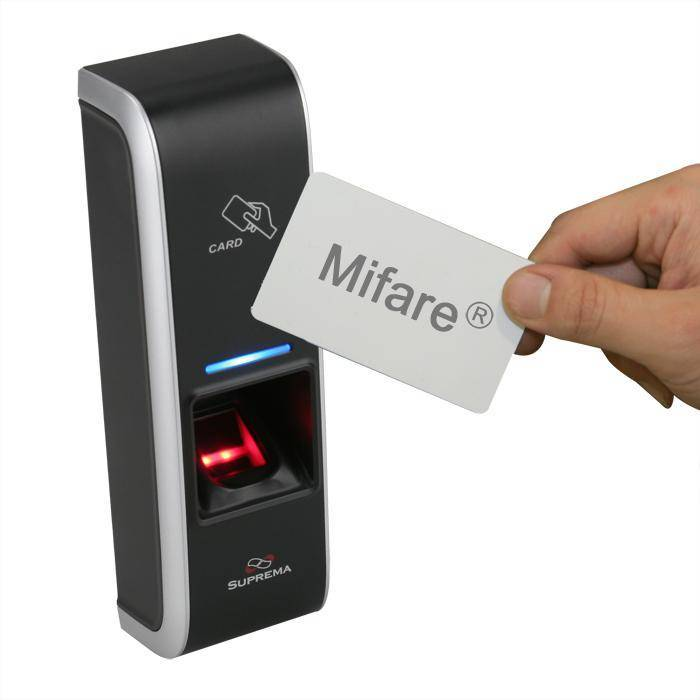
\includegraphics[width=5cm]{1.png}
\caption{Hình ảnh minh họa}
\end{center}
\end{figure}
\vspace{1cm}


Đây là một hệ thống cho phép người dùng có thể kiểm soát tự động giúp tiết kiệm nhân lực và nhanh chóng. Có thể áp dụng với việc điểm danh trong trường học, kiểm soát xe ra vào,...
\subsection{Phân tích đề tài và ý tưởng}
Thiết kế mô hình hệ thống điểm danh sinh viên bằng cách sử dụng thẻ từ với module SPI-RFID, hiển thị thông tin sinh viên lên LCD, đăng kí thông tin và cập nhật danh sách lên Web server.

\newpage
\section{Kiến trúc tổng quan của hệ thống}
\subsection{Chức năng module 1}
\textbf{NODE MCU – SERVER MODE (AP MODE)}\\
Cập nhật danh sách chứa thông tin của sinh viên (bao gồm tên và mã số sinh viên)
\vspace{1cm}
\begin{figure}[h!]
\begin{center}
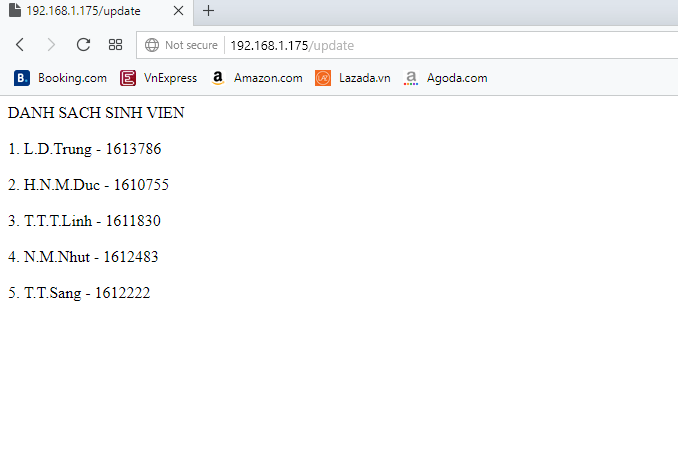
\includegraphics[width=10cm]{2.png}
\end{center}
\end{figure}
\vspace{1cm}
\subsection{Chức năng module 2}
\textbf{SPI RFID READER}\\
Sinh viên sử dụng thẻ quẹt lên đầu đọc thẻ, hệ thống sẽ tự động thu nhập thông tin đầu vào bao gồm: mã thẻ, tên và mã số sinh viên(nếu có).
\vspace{1cm}
\begin{figure}[h!]
\begin{center}
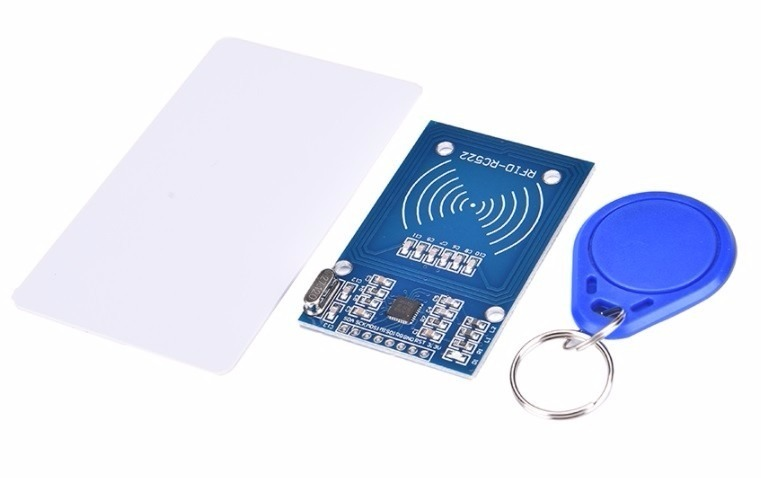
\includegraphics[width=10cm]{3.png}
\end{center}
\end{figure}
\vspace{1cm}
\subsection{Chức năng module 3}
\textbf{INTERFACE I2C LCD}\\
Sau khi sinh viên quẹt thẻ, nếu thẻ đã được đăng kí trước thì LCD sẽ hiển thị thông tin sinh viên\\

\vspace{1cm}
\begin{figure}[h!]
\begin{center}
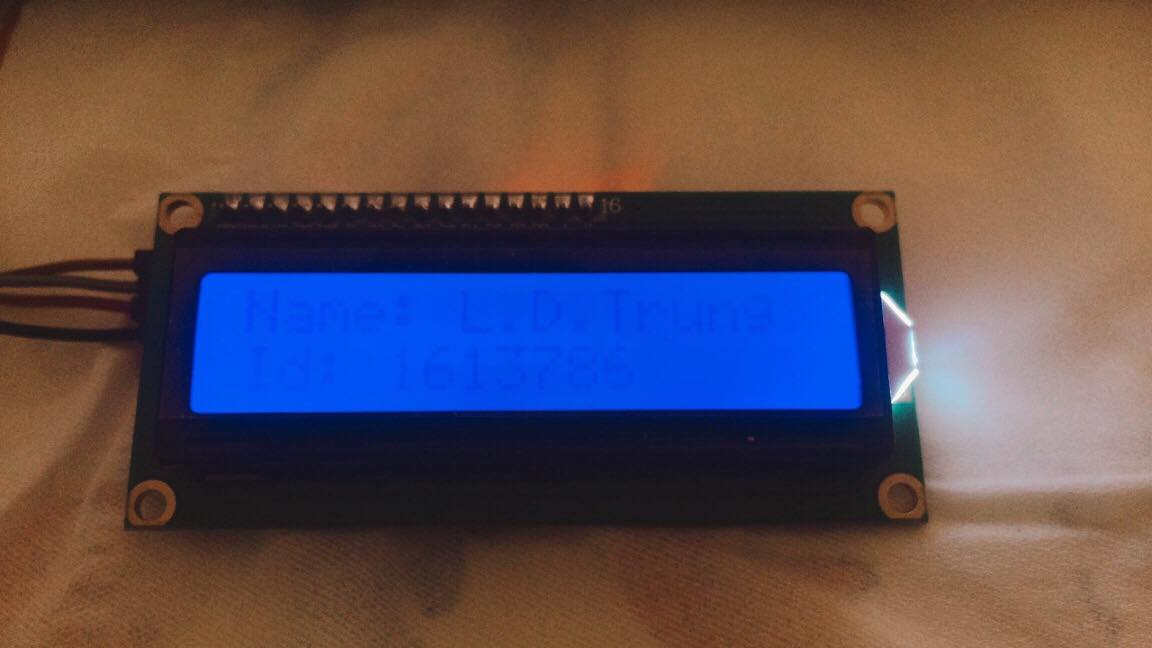
\includegraphics[width=10cm]{4.png}
\end{center}
\end{figure}
\vspace{1cm}

Nếu thẻ chưa được đăng kí thì hệ thống sẽ hiển thị "No Information"

\vspace{1cm}
\begin{figure}[h!]
\begin{center}
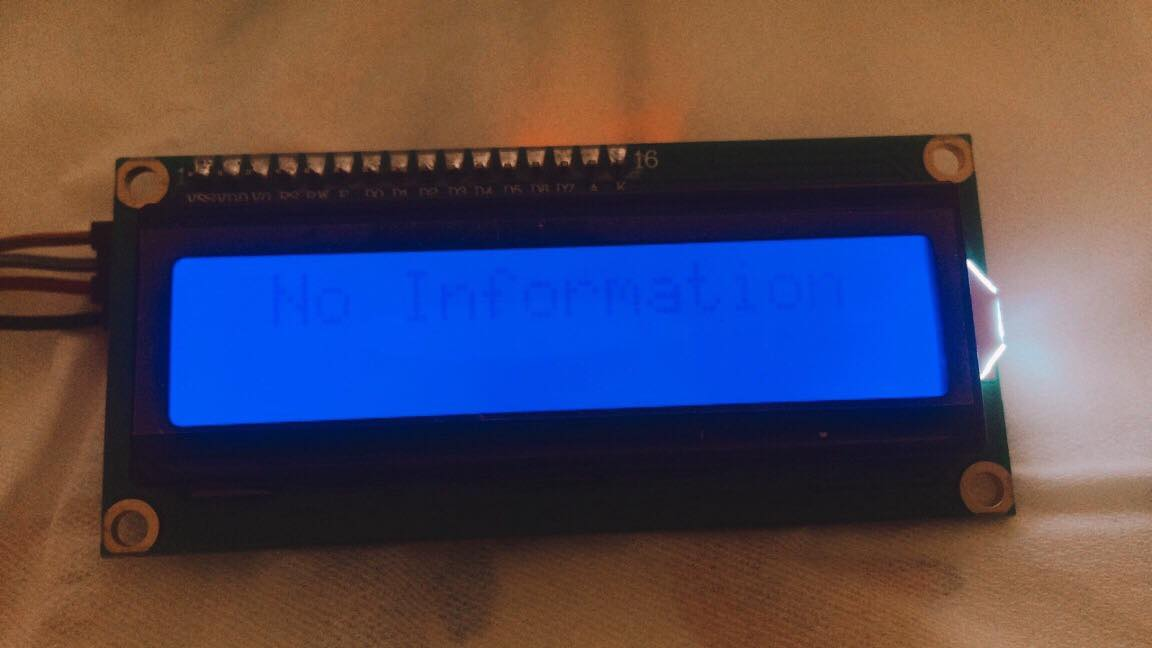
\includegraphics[width=10cm]{5.png}
\end{center}
\end{figure}
\vspace{1cm}
\subsection{Chức năng ngoài}
Nếu muốn đăng kí tài khoản mới thì sinh viên sử dụng 1 thẻ mới, bấm vào nút đăng kí và điền thông tin của mình. Hệ thống sẽ tự cập nhật danh sách sau đó. 
\newpage
\section{Hiện thực hệ thống}
\subsection{Sơ đồ máy trạng thái của hệ thống}
\vspace{1cm}
\begin{figure}[h!]
\begin{center}
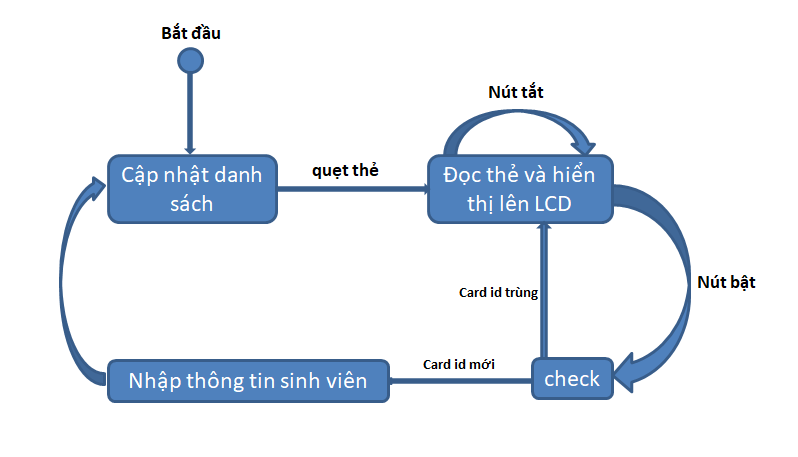
\includegraphics[width=15cm]{6.png}
\end{center}
\end{figure}
\vspace{1cm}
\subsection{Một số hàm xử lý chính của mỗi trạng thái}
\begin{itemize}
\item Cập nhật danh sách


\begin{figure}[h!]
\begin{center}
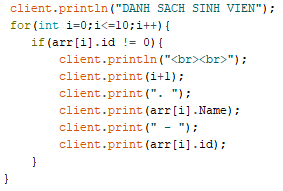
\includegraphics[width=7cm]{7.png}
\end{center}
\end{figure}


Sử dụng lệnh \textit{client.print} để in ra thông tin sinh viên trên web server.
\newpage
\item Đọc thẻ và hiển thị lên LCD

\begin{figure}[h!]
\begin{center}
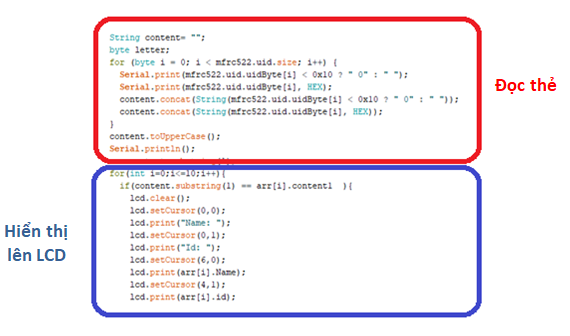
\includegraphics[width=15cm]{8.png}
\end{center}
\end{figure}

\item Check card id để xác định thẻ có phù hợp để đăng kí.
\begin{figure}[h!]
\begin{center}
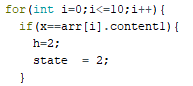
\includegraphics[width=7cm]{9.png}
\end{center}
\end{figure}

\item Nhập thông tin 
\begin{figure}[h!]
\begin{center}
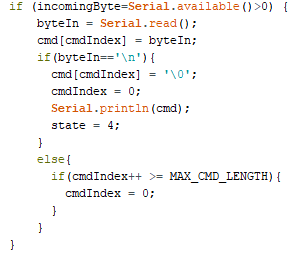
\includegraphics[width=7cm]{10.png}
\end{center}
\end{figure}



\end{itemize}
\newpage
\section{Tổng kết và Hướng mở rộng}
\subsection{Tổng kết}
Trong thời gian thực hiện bài tập cùng với sự giúp đỡ, hướng dẫn từ giảng viên và vận dụng những kiến thức có được trong quá trình làm các bài lab em đã có thể hoàn thành bài. Tuy nhiên do năng lực chuyên môn có hạn nên hệ thống có thể không đạt hết được yêu cầu. Em mong có thể nhận được những góp ý của thầy để bài có thể được hoàn thiện hơn.
\subsection{Hướng mở rộng}
Hiện nay việc kiểm soát tự động rất phổ biến và có nhiều ứng dụng trong đời sống. Từ hệ thống này có thể ứng dụng trong việc điểm danh trong trường học, chấm điểm công việc, ra vào trong nhà xe,.. Ngoài ra, có thể sử dụng vân tay hoặc nhân diện khuôn mặt bằng camera để nâng cao tính chặt chẽ...


%%%%%%%%%%%%%%%%%%%%%%%%%%%%%%%%%

\end{document}

